\subsection*{9.1 \& 9.2}
Perfectly competitive markets have 5 assumptions or characteristics.
\begin{enumerate}
    \item All agents within the market are price takers. They cannot influence the price of the good or service.
    \item There are many buyers and sellers in the marketplace.
    \item The product is homogeneous. Everybody in the industry is selling identical products.
    \item There are no barriers to entry or exit. Firms can enter or exit the market freely.
    \item Information is perfect. You may not be fully informed, but what you know, everyone else knows. Equally informed.
\end{enumerate}
Examples of perfectly competitive markets are agriculture and financial markets.
\begin{figure}[H]
    \centering
    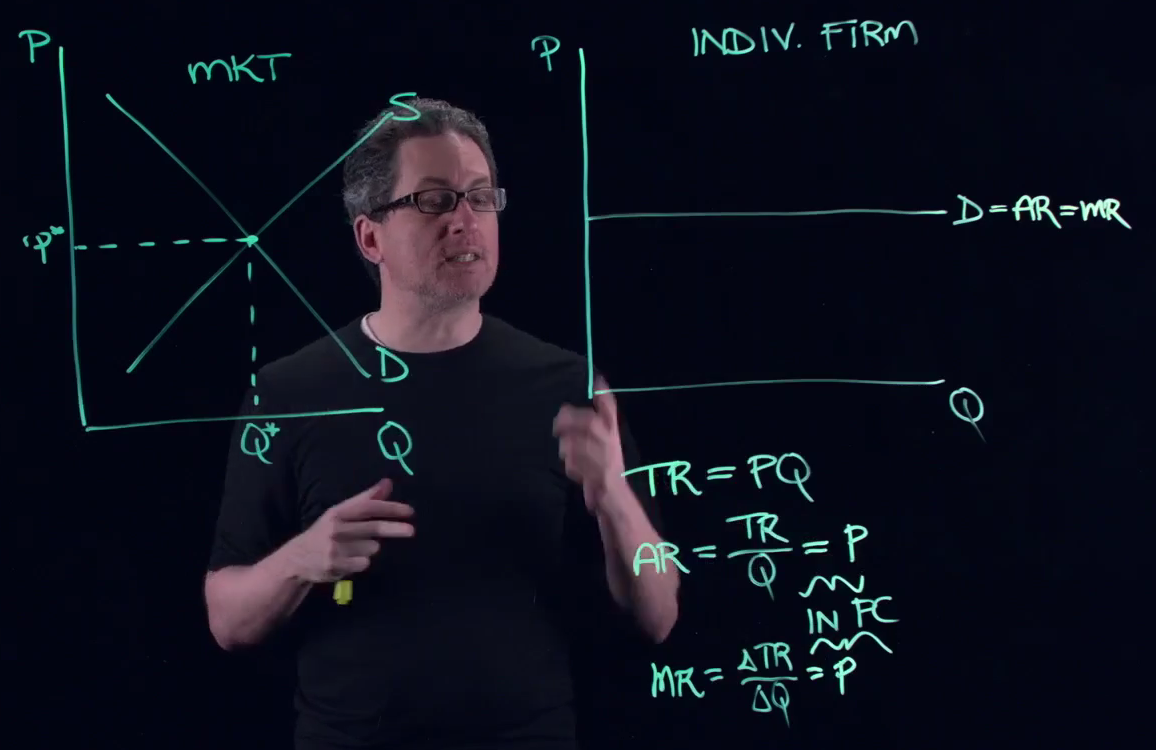
\includegraphics[width=0.5\textwidth]{./Chapter9/PerfectlyCompetitive.png}
    \caption{Perfectly Competitive Market}
\end{figure}
\par
Remember that Total Revenue (TR) is price times quantity.\\
Average Revenue (AR) is TR divided by quantity. In other words Average Revenue is equal to price (in a perfectly competitive market).\\
Marginal Revenue (MR) is the change in Total revenue divided by the change in quantity. In other words, Marginal Revenue is equal to price (in a perfectly competitive market).